\clearpage
\section{PC} \label{sec:PC}

\begin{figure}[H]
\centering
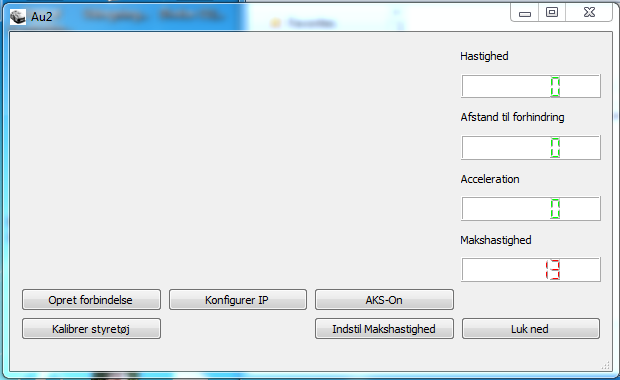
\includegraphics[width=\textwidth* 3/4,height=\textwidth* 9/20 ]{../fig/billeder/gui_start.png}
\caption{GUI hovedvindue}
\label{fig:GUI_hovedvindue}
\end{figure}

\subsection{Sekvensdiagrammer}

I denne sektion beskrives sekvensdiagrammer over usecasene for GUI'en. Der er valgt at lave i alt 4 scenarier af UC1 hvor 3 af dem inkluderer fejl. Dette er gjort for at gøre det mere overskueligt, da et sekvensdiagram med en masse undtagelser hurtigt bliver forvirrende.På figur
\ref{fig:cd_uc1_succes_gui} ses sekvensdiagrammet over UC1 scenarie: succes.

\subsubsection{UC1 Succes}

\begin{figure}[H]
\centering
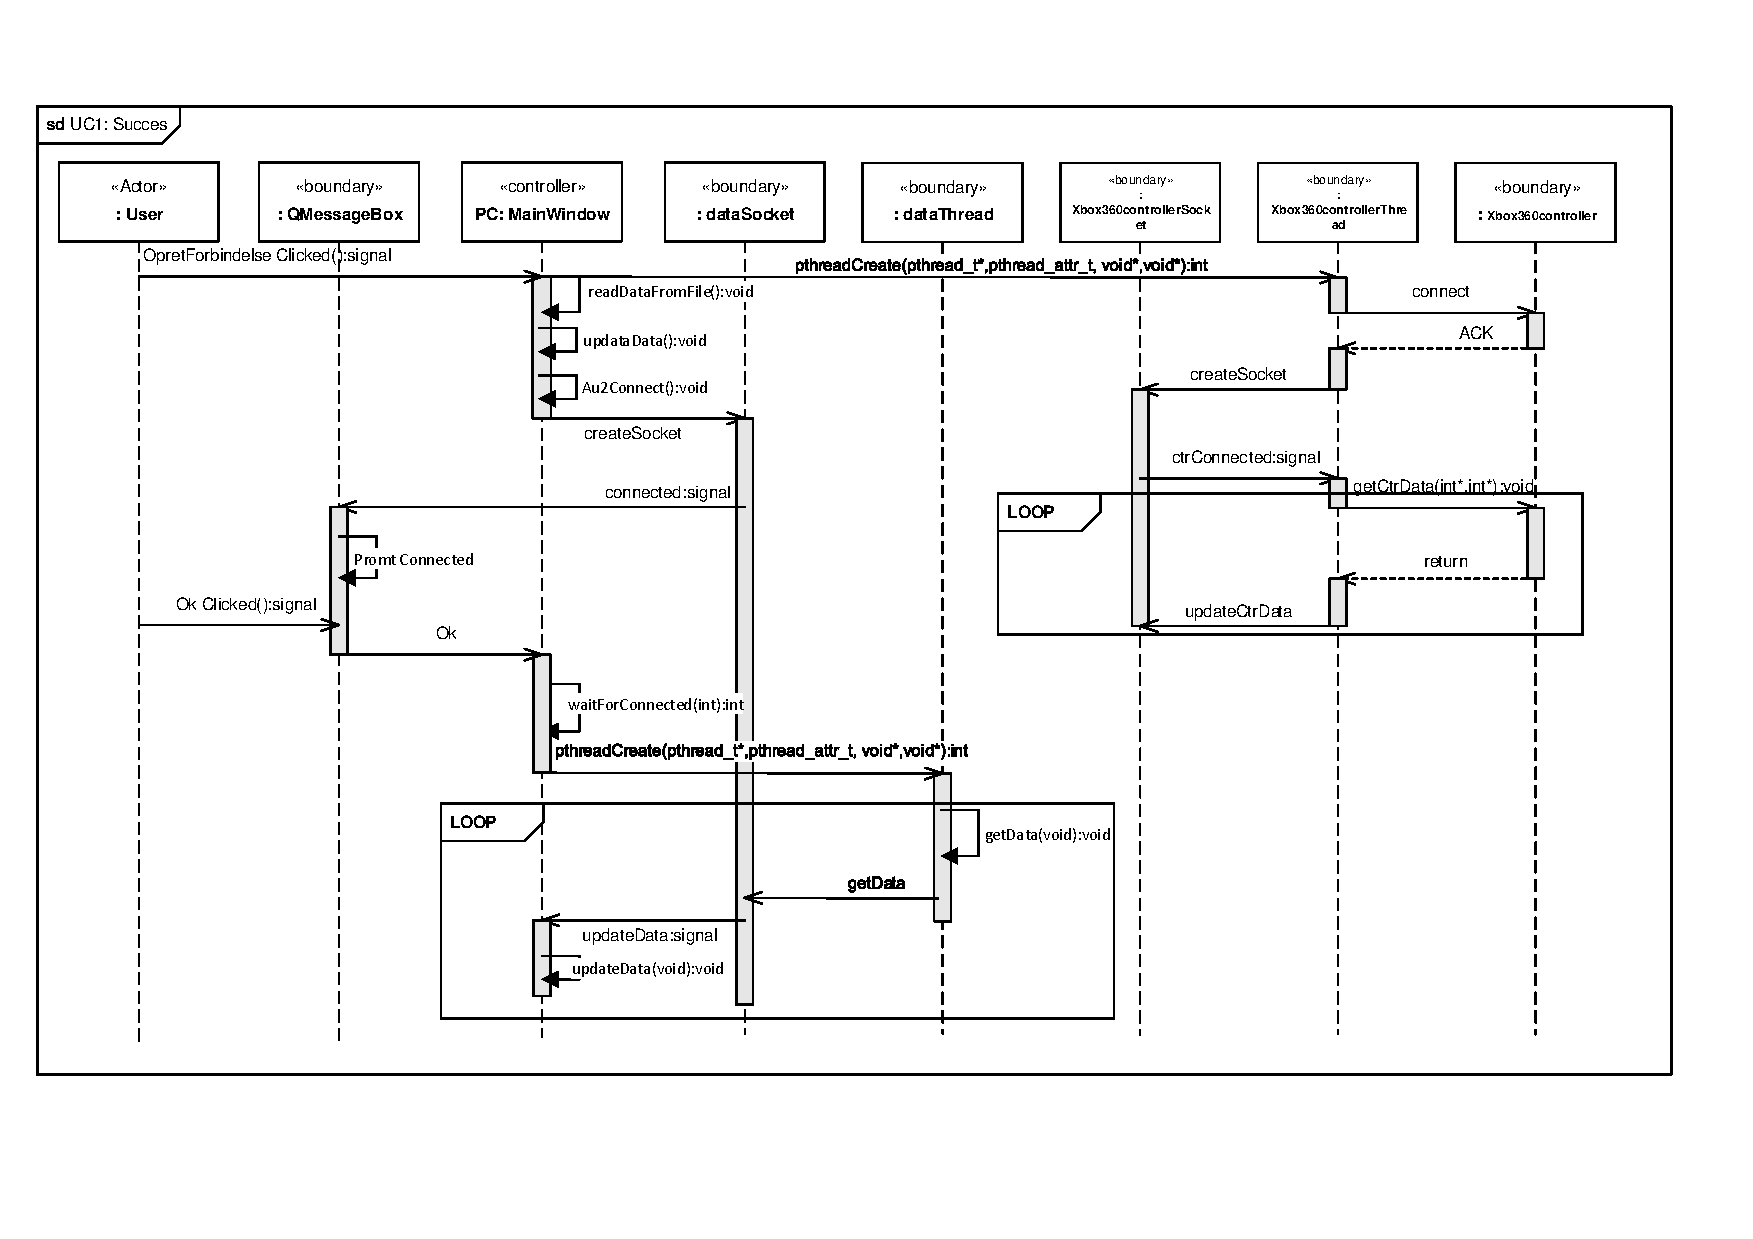
\includegraphics[width=\textwidth* 1,height=\textwidth* 7/10 ]{../fig/diagrammer/pc/sd_uc1_succes.pdf}
\caption{Sekvensdiagram over UC1 senarie:succes}
\label{fig:cd_uc1_succes_gui}
\end{figure}

Når usecasen startes klikker brugeren på ''Opret forbindelse'' på GUI'en. Herefter vil MainWindow starte Xbox360ControllerThread, som vil oprette en socketforbindelse mellem bilen og PC til at sende controllerdata. Efterfølgende vil MainWindow indlæse data, som blev gemt i en fil sidste gang programmet lukkede ned og derefter opdatere vinduet. Nu vil MainWindow oprette en socket mere til at sende og modtage data fra og til bilen. Når socketforbindelsen er oprettet vil dataSocket sende et signal til MainWindow, som derved vil promte brugeren at forbindelsen er oprettet. Se figur \ref{fig:GUI_uc1_success}. Når brugeren lukker vinduet ved at klikke ''Ok'' venter MainWindow på at der er forbindelse for at derefter oprette dataThread som efterfølgende vil stå for at opdatere vinduet med hastig, afstand, acceleration osv. Det virker måske lidt dumt at vente på at der er forbindelse efter at der er givet signal om der er forbindelse. Dette skyldes at når brugeren trykker på ''Ok'' sættes en variabel til 1. Hvis forbindelsen senere mistes sættes denne variabel til 0, således dataThread ikke skriver til en socketforbindelse som ikke længere er aktiv. Ventetiden er for at sikre at signalet kommer inden for en given tid. Defor: Kommer signalet om at forbindelsen ikke er oprettet inden for en given tid, vil programmet lave en fejl som det ses i figur \ref{fig:GUI_uc1_error_1}. Når dataThread har opdateret dataen, vil den give et signal til MainWindow om at der skal hentes nye data fra bilen. Det er derfor MainWindow som henter og sender data, men dataThread som opdatere selve dataen på GUI'en. Dette skyldes at QTcpsocket ikke kan køres i en separat tråd som det gøres med Xbox360ControllerThread hvis der skal gives signaler. Der sker derfor en fejl i programmet når Xbox360 controlleren er forbundet og TCP forbindelsen mistes. Der har desværre ikke været tid til at finde en løsning på dette problem.  

\begin{figure}[H]
\centering
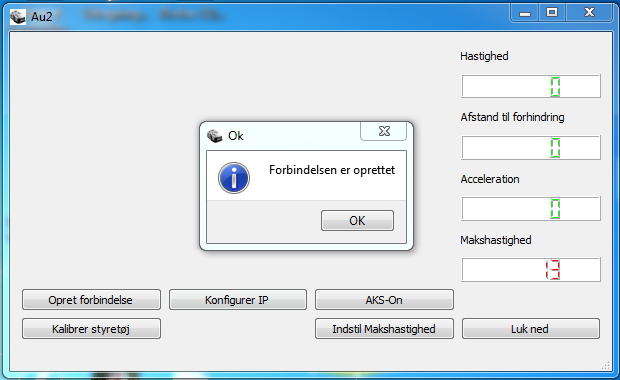
\includegraphics[width=\textwidth* 3/4,height=\textwidth* 9/20 ]{../fig/billeder/gui_uc1_success.png}
\caption{GUI UC1 succes}
\label{fig:GUI_uc1_success}
\end{figure}


\subsubsection{UC1 Error 1: Forbindelse kunne ikke oprettes}
I denne sektion beskrives fejlen, at der ikke kan oprettes forbindelse til bilen. Dette bliver som før beskrevet konkluderet i WaitForConnected(), som venter 1 sekund. Er der ikke givet signal inden deletes dataSocket og Xbox360ControllerSocket. Brugeren promtes med at forbindelsen ikke kunne oprettes. Se sekvensdiagrammet i figur \ref{fig:cd_uc1_error_1} og advarselsskiltet i figur \ref{fig:GUI_uc1_error_1}

\begin{figure}[H]
\centering
\includegraphics[width=\textwidth* 1,height=\textwidth* 7/10 ]{../fig/diagrammer/pc/sd_uc1_Error_1.pdf}
\caption{Sekvensdiagram over UC1 senarie:Error 1}
\label{fig:cd_uc1_error_1}
\end{figure}

\begin{figure}[H]
\centering
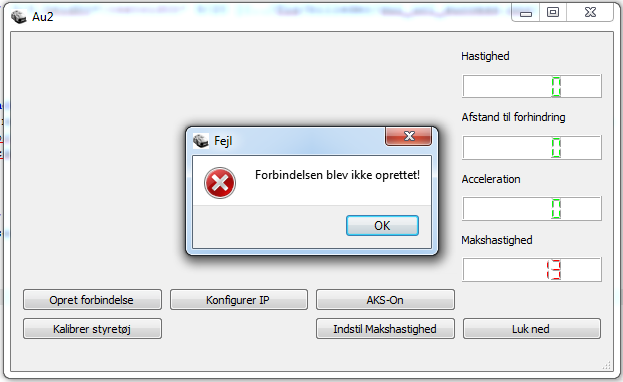
\includegraphics[width=\textwidth* 3/4,height=\textwidth* 9/20 ]{../fig/billeder/gui_uc1_error_1.png}
\caption{GUI UC1 Error 1}
\label{fig:GUI_uc1_error_1}
\end{figure}

\subsubsection{UC1 Error 2: Controller er ikke forbundet}
I denne sektion beskrives fejlen, at Xbox360-controlleren ikke er forbundet til PC'en. Når Xbox360controllerThread oprettes vil den spørge om controlleren er tilsluttet. Hvis den ikke er promtes bruger med at controlleren ikke er forbundet. Se sekvensdiagrammet i figur \ref{fig:cd_uc1_error_2} og advarselsskiltet i figur \ref{fig:GUI_uc1_error_2}

\begin{figure}[H]
\centering
\includegraphics[width=\textwidth* 1,height=\textwidth* 7/10 ]{../fig/diagrammer/pc/sd_uc1_Error_2.pdf}
\caption{Sekvensdiagram over UC1 senarie:Error 2}
\label{fig:cd_uc1_error_2}
\end{figure}

\begin{figure}[H]
\centering
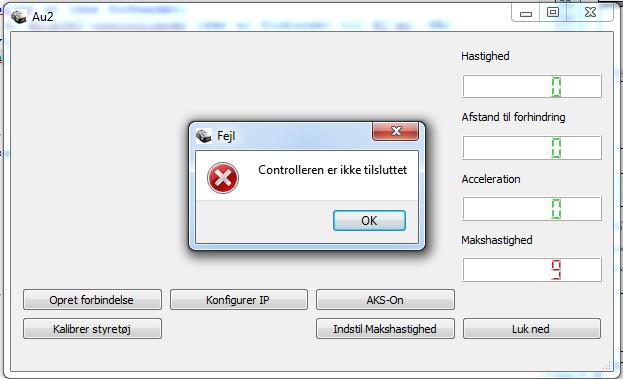
\includegraphics[width=\textwidth* 3/4,height=\textwidth* 9/20 ]{../fig/billeder/gui_uc1_error_2.png}
\caption{GUI UC1 Error 1}
\label{fig:GUI_uc1_error_2}
\end{figure}

\subsubsection{UC1 Error 3: Forbindelsen bliver afbrudt}
I denne sektion beskrives fejlen, at forbindelsen mellem bil og PC pludselig bliver afbrudt. dataSocket giver signal til MainWindow om at forbindelsen er afbrudt, som herefter giver besked til brugeren. Herefter stopper dataSocket med at opdatere data. Er controlleren forbundet og bliver denne forbindelse også afbrudt crasher programmet desværre. Denne fejl er beskrevet tidligere. Se sekvensdiagrammet i figur \ref{fig:cd_uc1_error_3} og advarselsskiltet i figur \ref{fig:GUI_uc1_error_3} 

\begin{figure}[H]
\centering
\includegraphics[width=\textwidth* 1,height=\textwidth* 7/10 ]{../fig/diagrammer/pc/sd_uc1_Error_3.pdf}
\caption{Sekvensdiagram over UC1 senarie:Error 3}
\label{fig:cd_uc1_error_3}
\end{figure}

\begin{figure}[H]
\centering
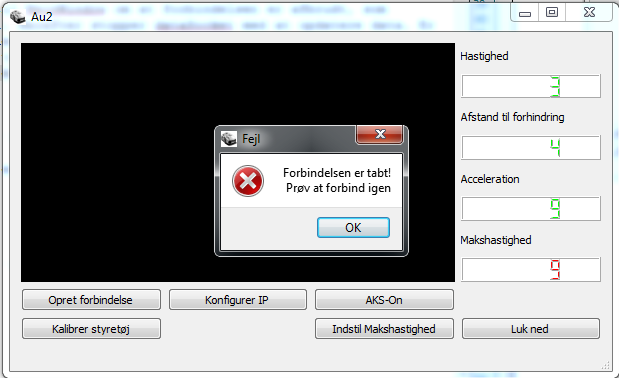
\includegraphics[width=\textwidth* 3/4,height=\textwidth* 9/20 ]{../fig/billeder/gui_uc1_error_3.png}
\caption{GUI UC1 Error 3}
\label{fig:GUI_uc1_error_3}
\end{figure}

\subsubsection{UC8: Konfigurer IP-adresse}
For at aktivere usecase 8 trykker bruger på ''Konfigurer IP''. Herefter åbner MainWindow en inputdialog som bruger indtaster IP-adressen i og efterfølgende trykker ''Ok''. Se sekvensdiagrammet i figur \ref{fig:cd_uc8} og indputdialogen i figur \ref{fig:GUI_uc8} 

\begin{figure}[H]
\centering
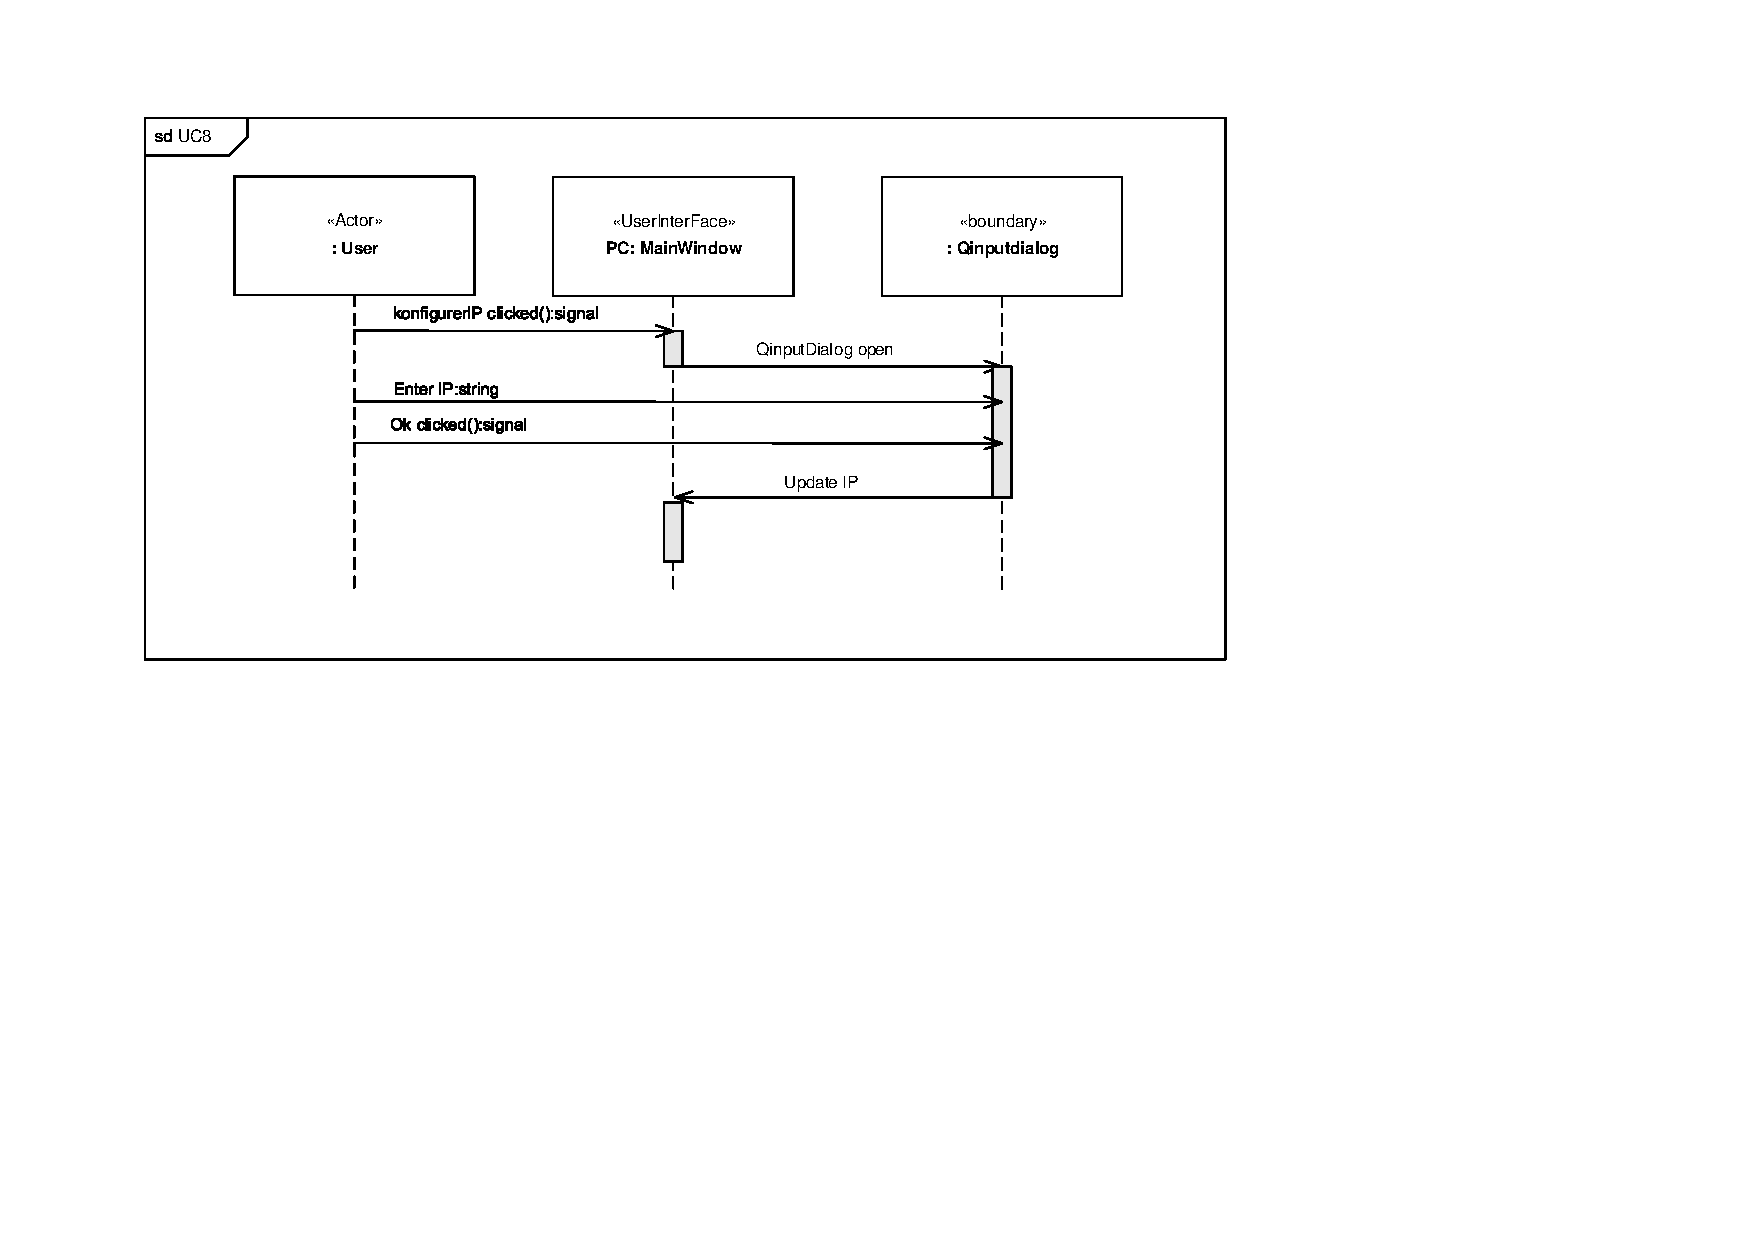
\includegraphics[width=\textwidth* 2/3,height=\textwidth* 4/10 ]{../fig/diagrammer/pc/sd_uc8.pdf}
\caption{Sekvensdiagram over UC8}
\label{fig:cd_uc8}
\end{figure}

\begin{figure}[H]
\centering
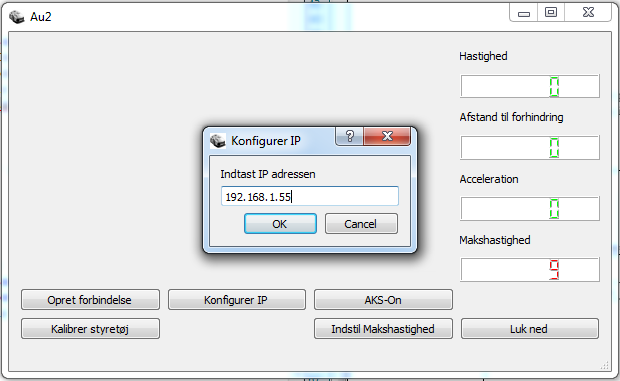
\includegraphics[width=\textwidth* 3/4,height=\textwidth* 9/20 ]{../fig/billeder/gui_uc8.png}
\caption{GUI UC8}
\label{fig:GUI_uc8}
\end{figure}

\subsubsection{UC9: Tænd/sluk AKS}
For at aktivere usecase 9 trykker bruger på ''AKS-On''.
Når bruger trykker på denne ændres teksten til ''AKS-Off''. Er teksten i forvejen ''AKS-Off'' ændres denne til ''AKS-On''. En variabel i MainWindow opdateres og gived med til bilen næste gang data bliver opdateret i UC1. Se sekvensdiagrammet i figur \ref{fig:cd_uc9} og indputdialogen i figur \ref{fig:GUI_uc9}

\begin{figure}[H]
\centering
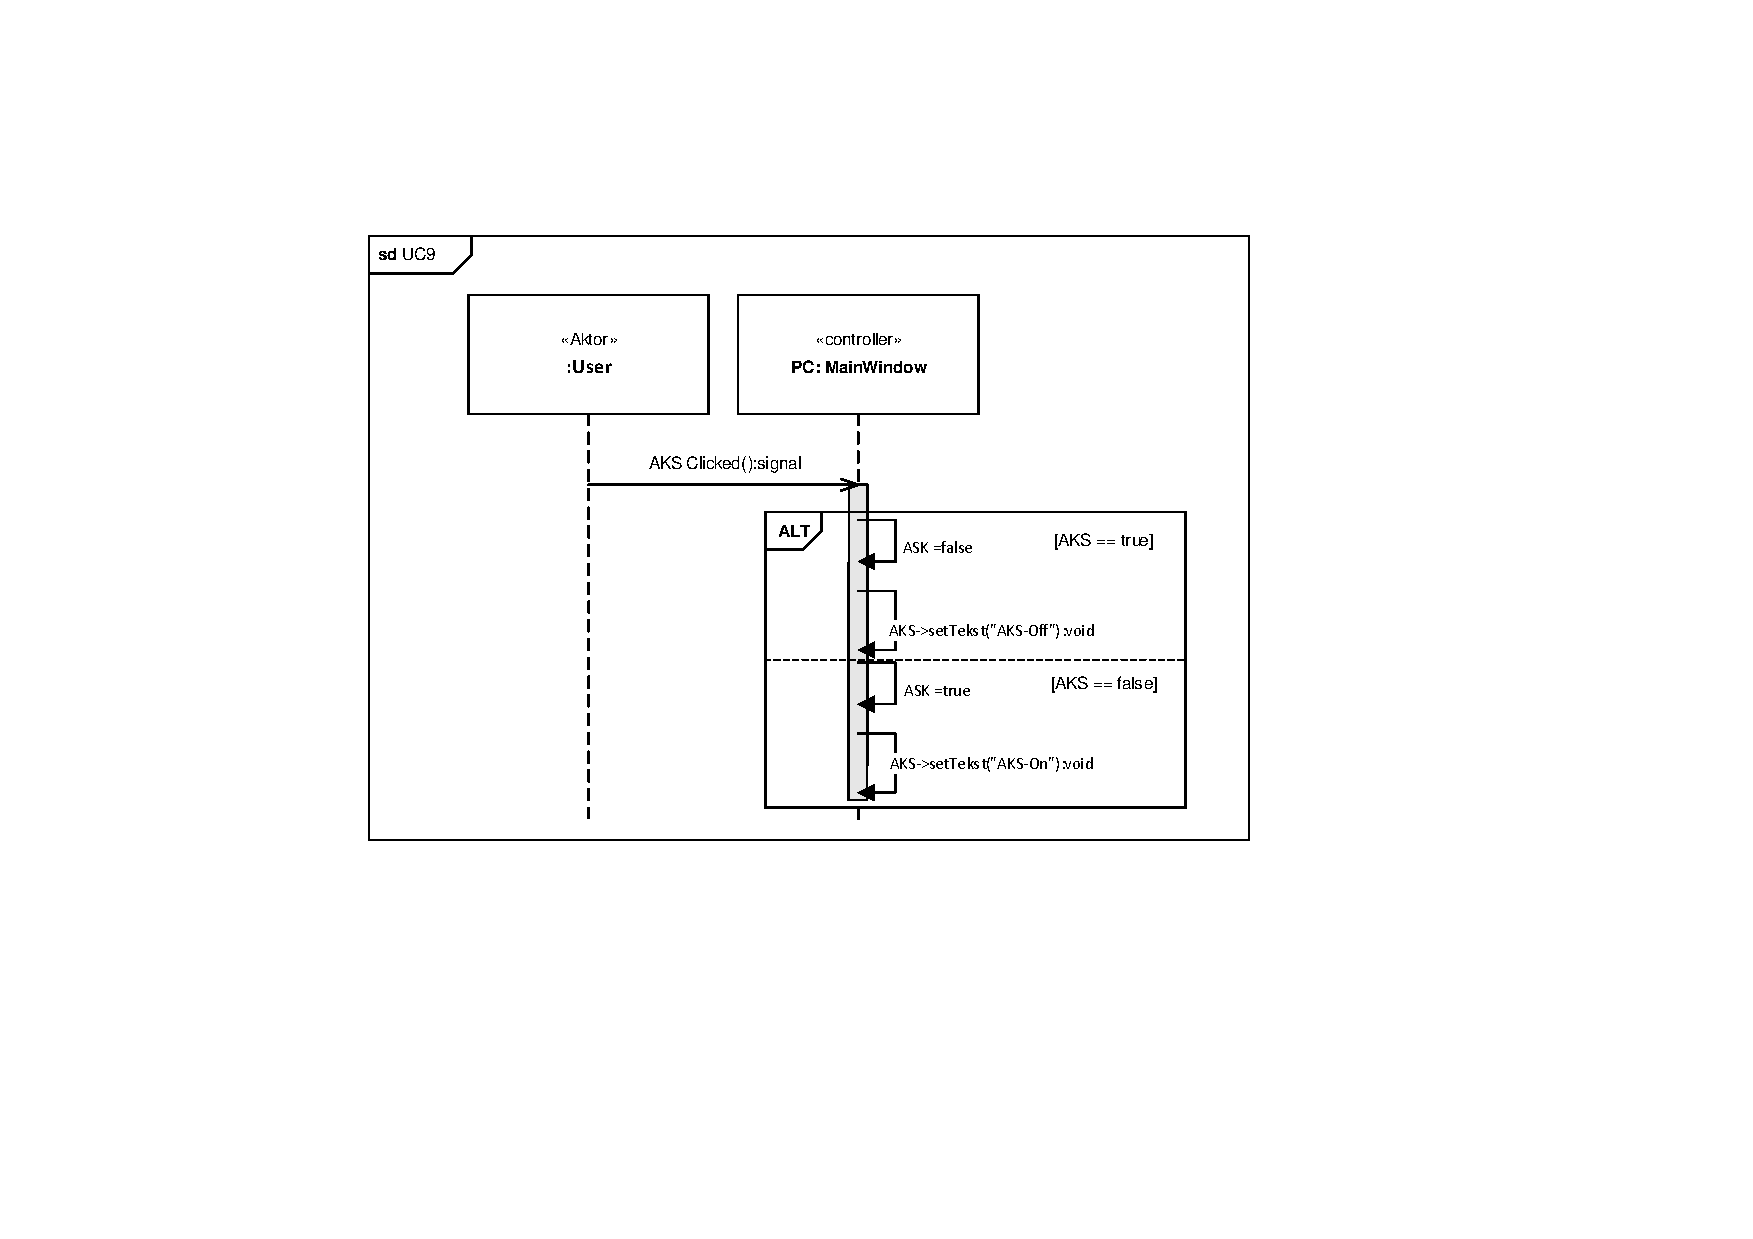
\includegraphics[width=\textwidth* 2/3,height=\textwidth* 4/10 ]{../fig/diagrammer/pc/sd_uc9.pdf}
\caption{Sekvensdiagram over UC9}
\label{fig:cd_uc9}
\end{figure}

\begin{figure}[H]
\centering
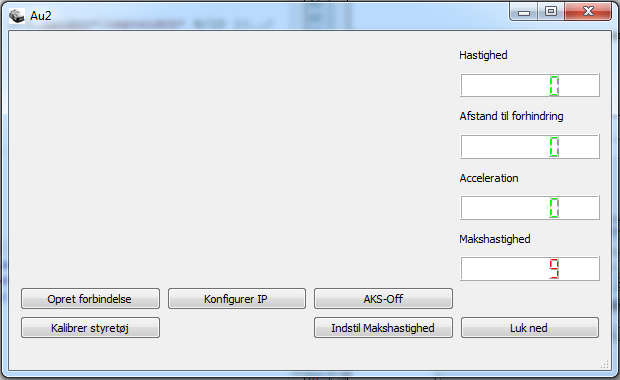
\includegraphics[width=\textwidth* 3/4,height=\textwidth* 9/20 ]{../fig/billeder/gui_uc9.png}
\caption{GUI UC9}
\label{fig:GUI_uc9}
\end{figure}

\subsubsection{UC10: Indstil makshastighed}
For at aktivere usecase 10 trykker bruger på ''Indstil makshastighed''.
MainWindow åbner en inputdialog hvor i bruger indtaster et tal mellem 0 og 10. Inputdialogen accepterer ikke indtastninger uden for dette interval. Se sekvensdiagrammet i figur \ref{fig:cd_uc10} og indputdialogen i figur \ref{fig:GUI_uc10}

\begin{figure}[H]
\centering
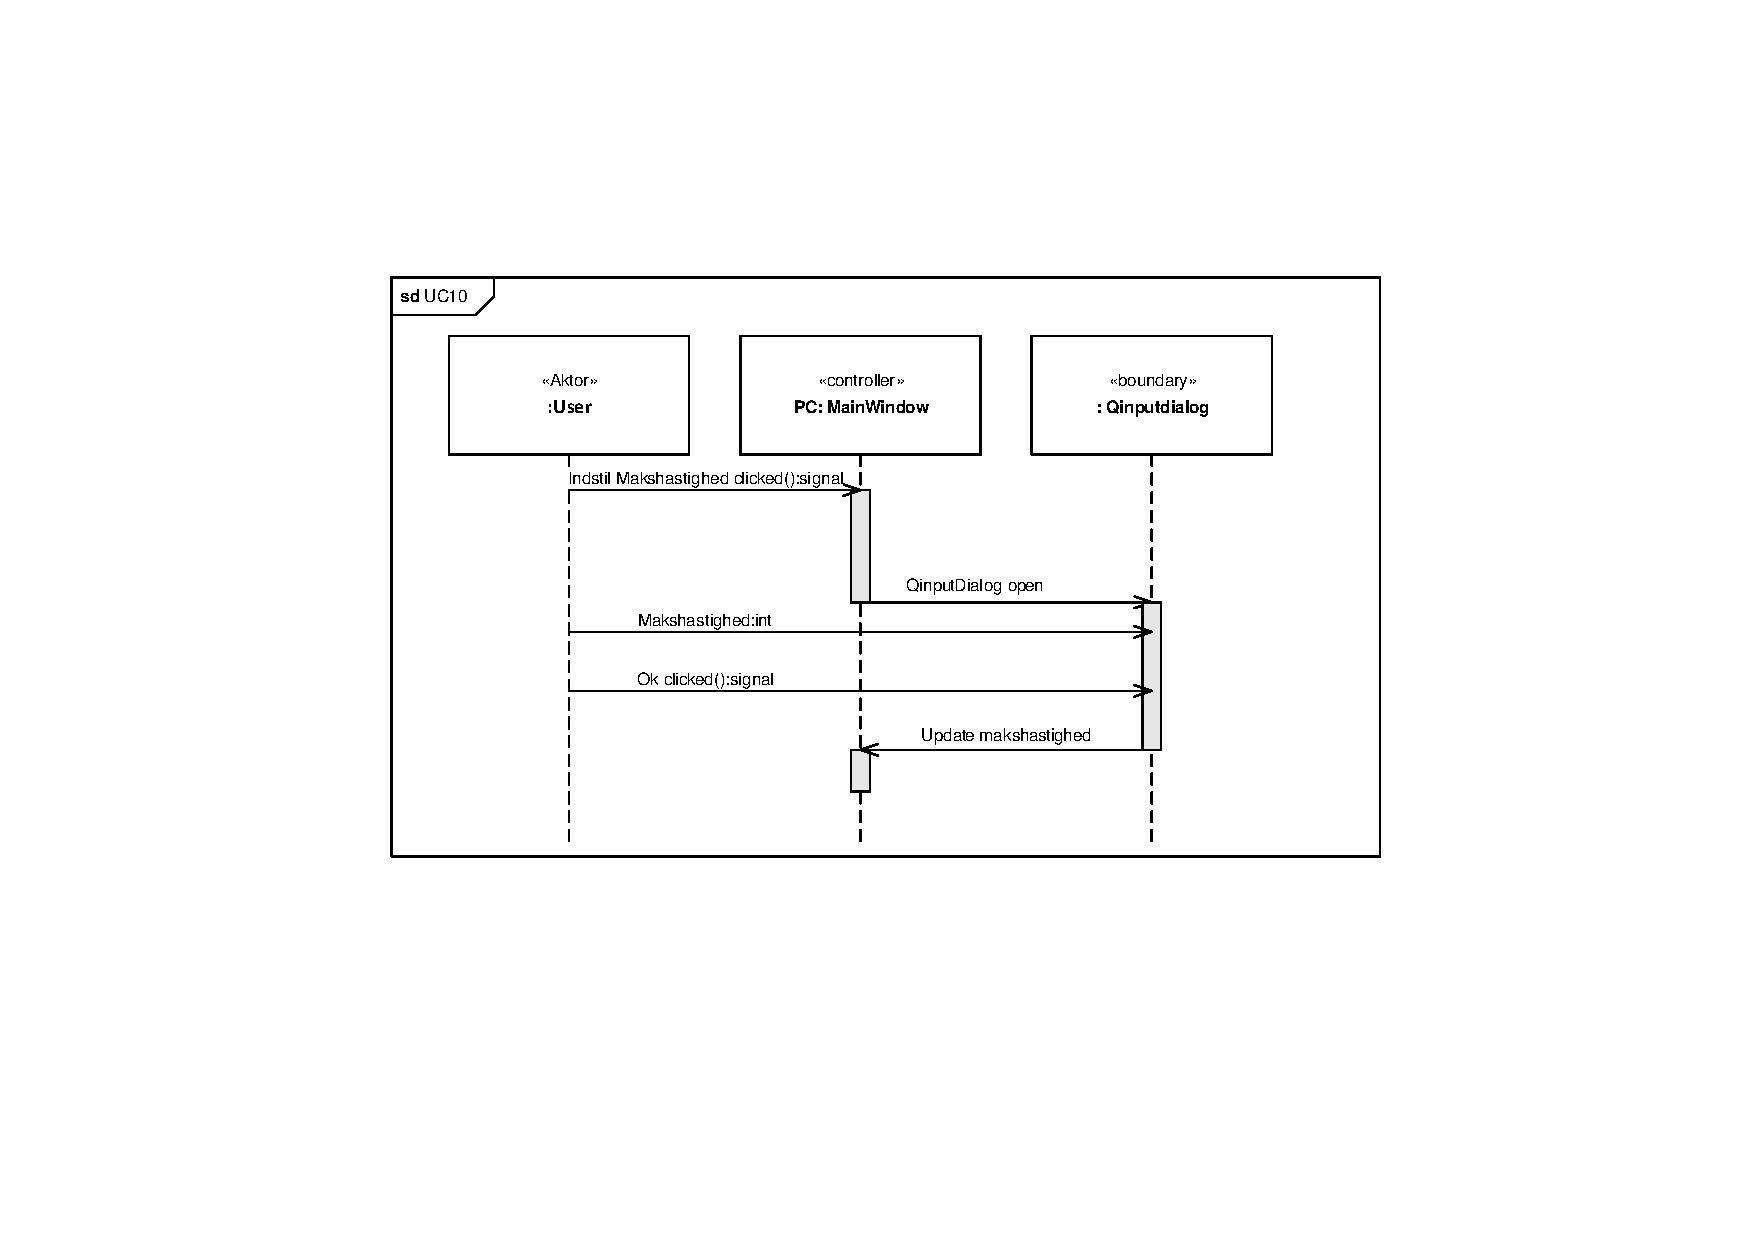
\includegraphics[width=\textwidth* 2/3,height=\textwidth* 4/10 ]{../fig/diagrammer/pc/sd_uc10.pdf}
\caption{Sekvensdiagram over UC10}
\label{fig:cd_uc10}
\end{figure}

\begin{figure}[H]
\centering
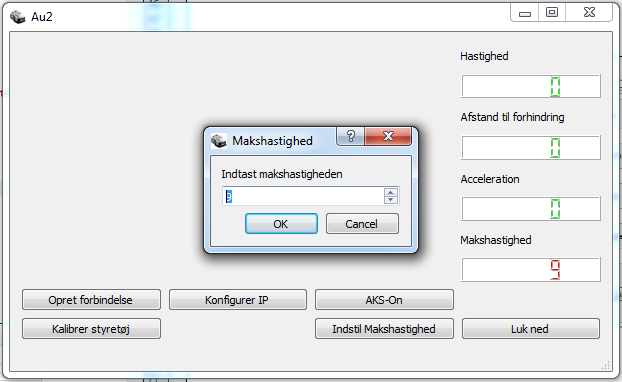
\includegraphics[width=\textwidth* 3/4,height=\textwidth* 9/20 ]{../fig/billeder/gui_uc10.png}
\caption{GUI UC10}
\label{fig:GUI_uc10}
\end{figure}

\subsubsection{UC11: Kalibrer styretøj}
For at aktivere usecase 11 trykker bruger på ''Kalibrer styretøj''.
MainWindow åbner en inputdialog hvor i bruger indtaster et tal mellem -50 og 50. Inputdialogen accepterer ikke indtastninger uden for dette interval. Se sekvensdiagrammet i figur \ref{fig:cd_uc11} og indputdialogen i figur \ref{fig:GUI_uc11}

\begin{figure}[H]
\centering
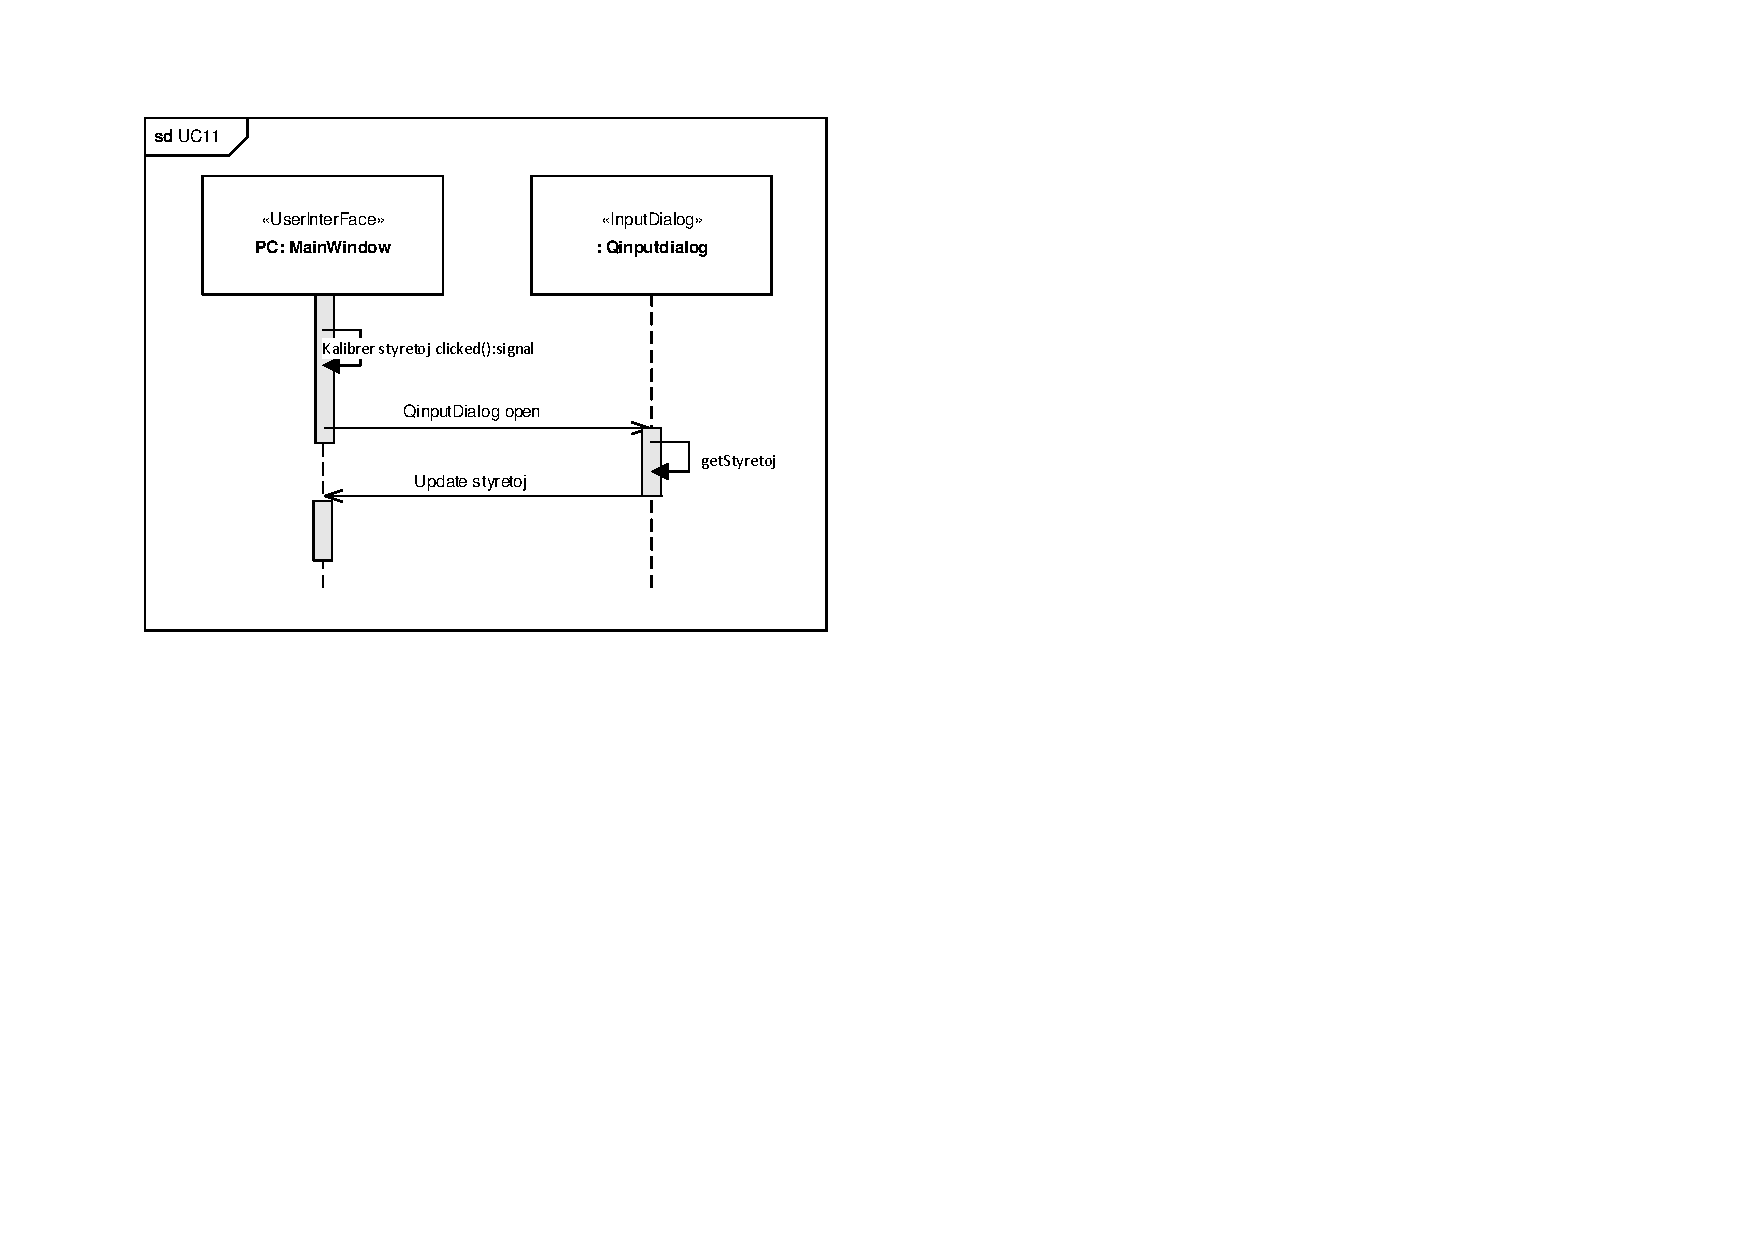
\includegraphics[width=\textwidth* 2/3,height=\textwidth* 4/10 ]{../fig/diagrammer/pc/sd_uc11.pdf}
\caption{Sekvensdiagram over UC11}
\label{fig:cd_uc11}
\end{figure}

\begin{figure}[H]
\centering
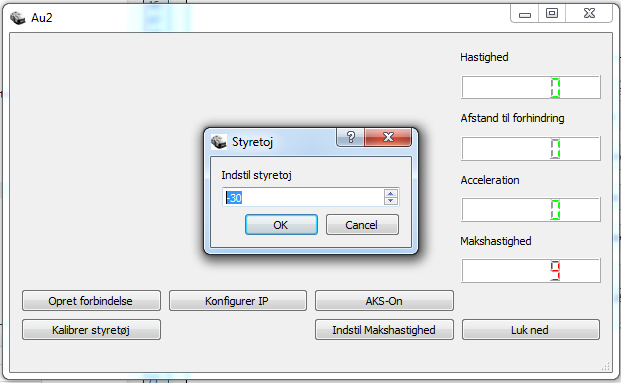
\includegraphics[width=\textwidth* 3/4,height=\textwidth* 9/20 ]{../fig/billeder/gui_uc11.png}
\caption{GUI UC11}
\label{fig:GUI_uc11}
\end{figure}

\subsubsection{UC12: Afbryd system}
For at aktivere usecase 11 trykker bruger på ''Luk ned''.
dataSocket beder bilen om at lukke ned og bilen svarer med et ACK. Modtages der ikke et ACK giver MainWindow bruger besked om at bilen ikke kan lukke ned. Se sekvensdiagrammet i figur \ref{fig:cd_uc11} og advarslen i figur \ref{fig:GUI_uc11}

\begin{figure}[H]
\centering
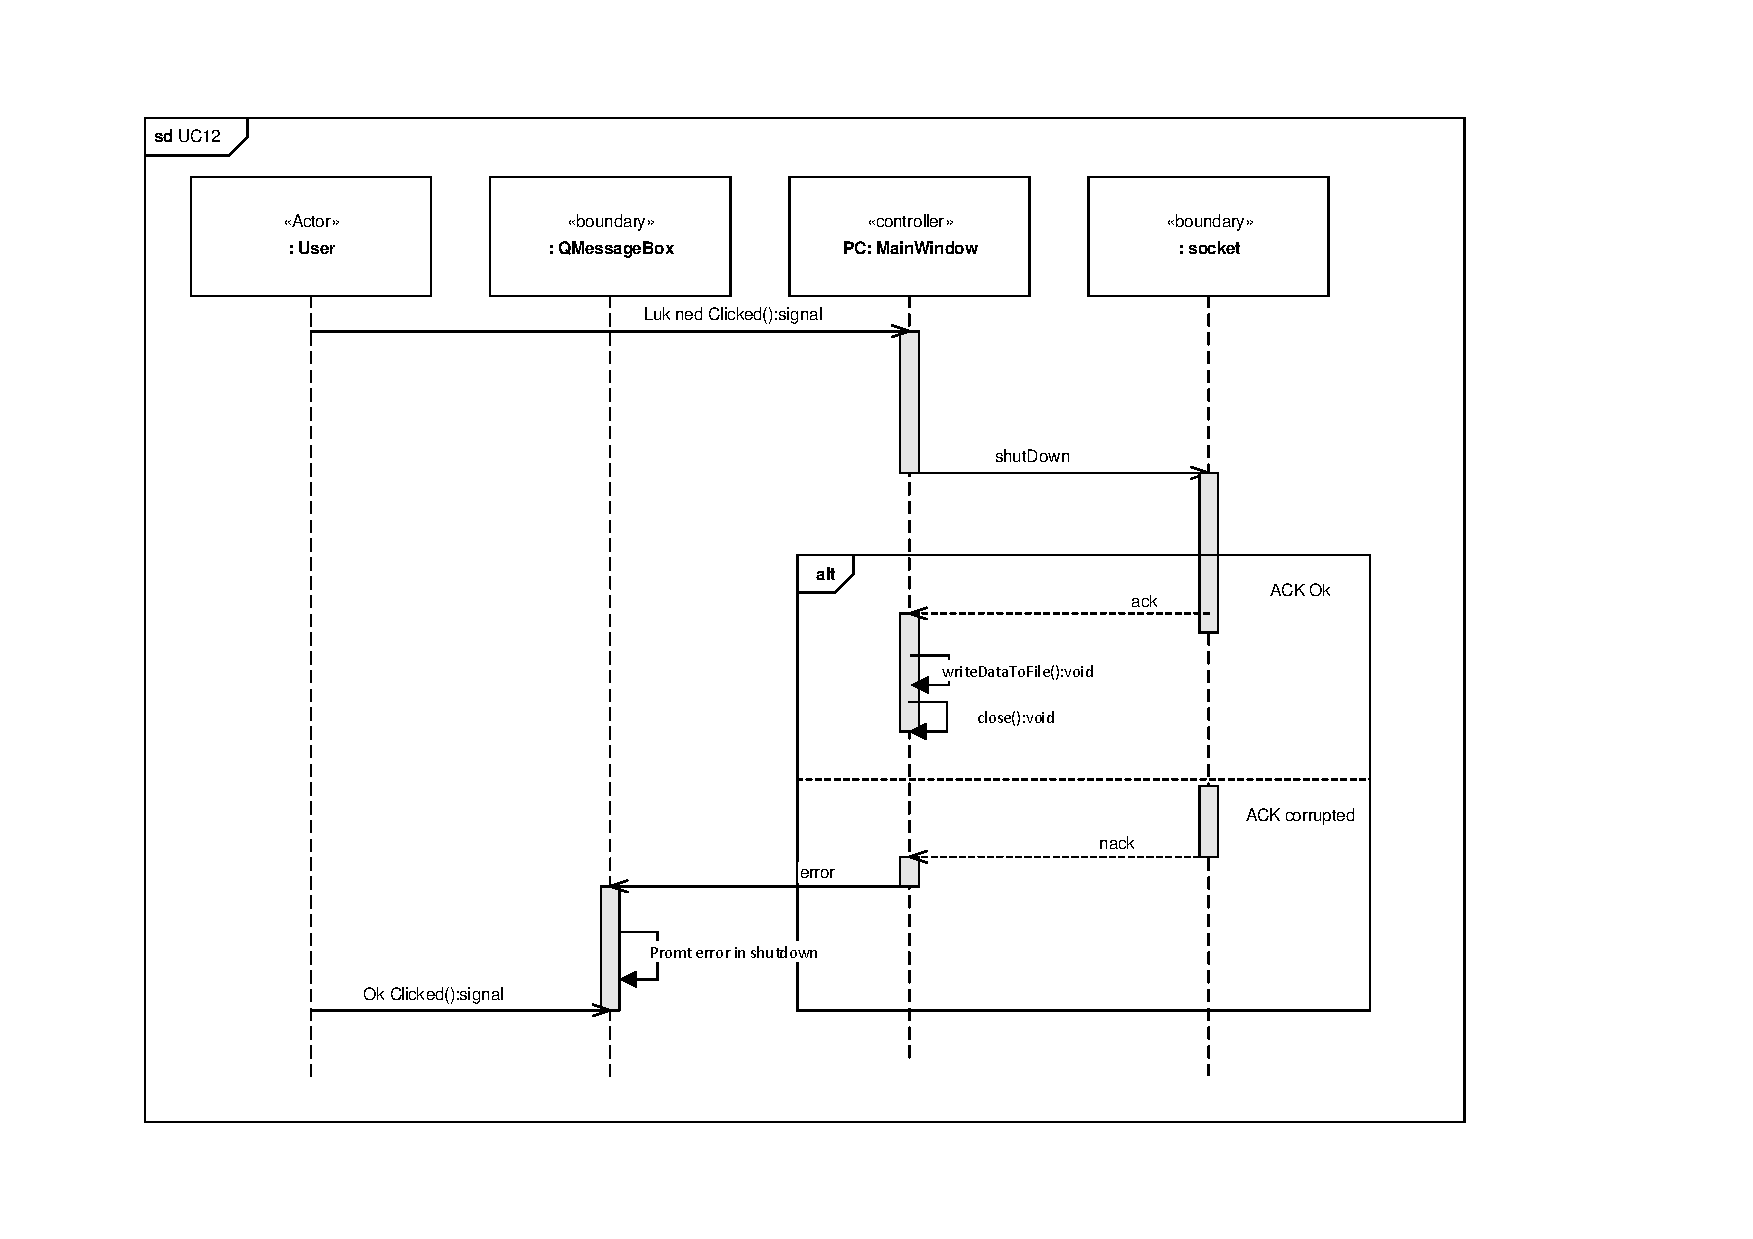
\includegraphics[width=\textwidth* 2/3,height=\textwidth* 4/10 ]{../fig/diagrammer/pc/sd_uc12.pdf}
\caption{Sekvensdiagram over UC12}
\label{fig:cd_uc12}
\end{figure}

\begin{figure}[H]
\centering
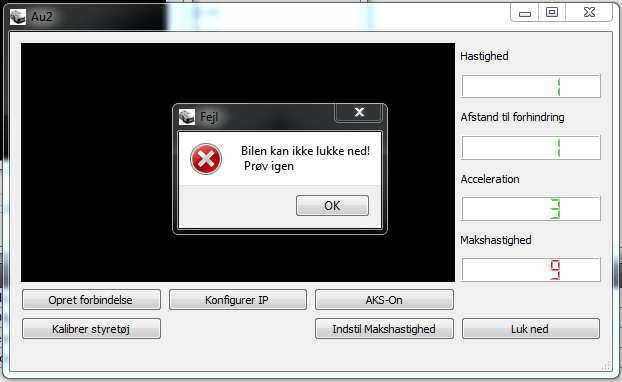
\includegraphics[width=\textwidth* 3/4,height=\textwidth* 9/20 ]{../fig/billeder/gui_uc12.png}
\caption{GUI UC12}
\label{fig:GUI_uc12}
\end{figure}


\subsection{Klassebeskrivelse}
I denne sektion vil der blive beskrevet klassen MainWindow og XboxController. MainWindow er GUI'ens hoved klasse hvor i alt styres fra. XboxController er controllerens klasse som MainWindow bruger til at streame controllerdata fra.

\begin{figure}[H]
\centering
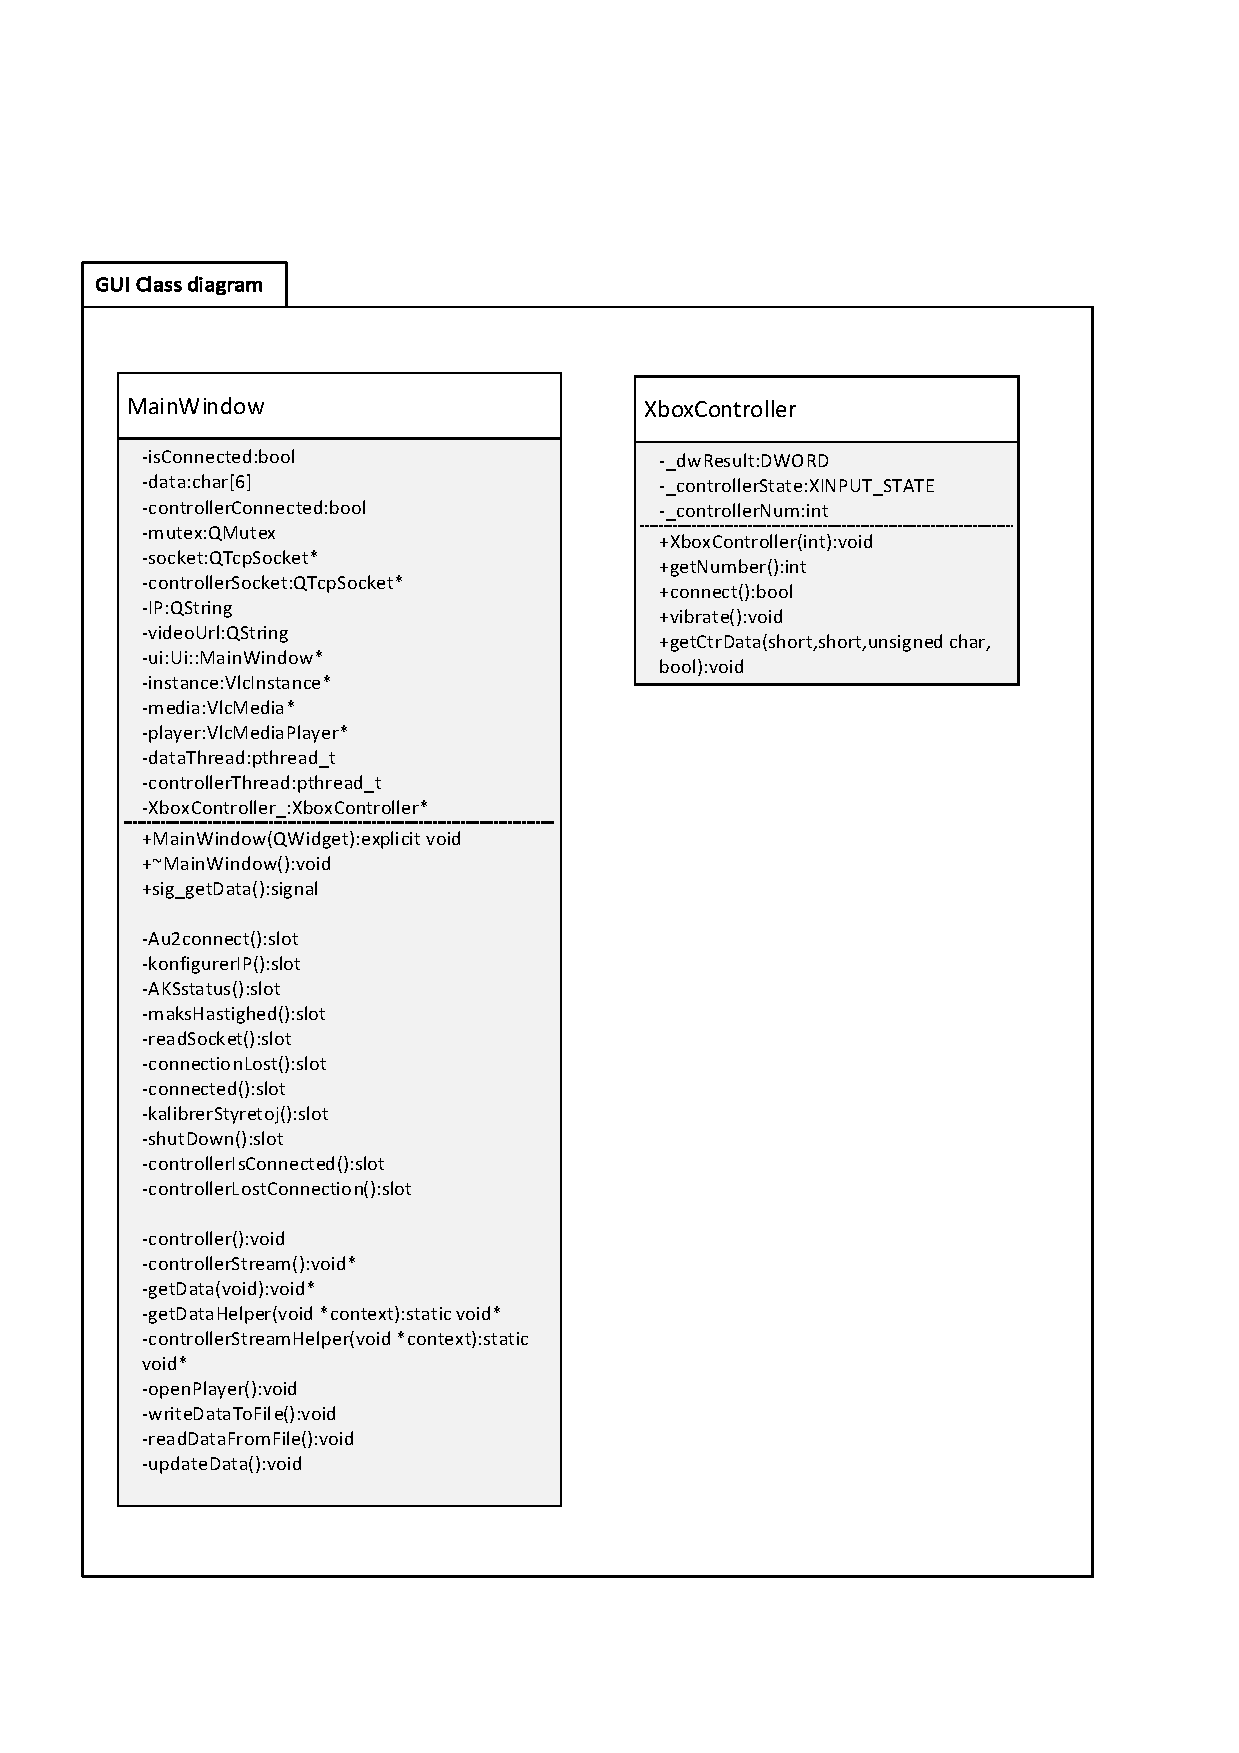
\includegraphics[width=\textwidth* 9/10]{../fig/diagrammer/pc/gui_classdiagram.pdf}
\caption{Klasse diagram over GUI}
\label{fig:cd_gui}
\end{figure}

\textbf{Attributter for MainWindow}

\begin{table}[H]
\begin{tabularx}{\textwidth}{| Z | Z | L{10cm} |} \hline
Navn & Type & Beskrivelse \\\hline
\texttt{isConnected}         & \texttt{bool}           &Bliver brugt til at angive om socket har forbindelse til bilen eller ej \\\hline
\texttt{data}                & \texttt{char[6]}        &Char array som indeholder: Hastighed, Makshastighed, AKS-status, Styretøj, Acceleration og Afstand\\\hline
\texttt{controller -Connected} & \texttt{bool}           &Bruges til at angive om Xbox360-controlleren er forbundet eller ej\\\hline
\texttt{mutex}               & \texttt{QMutex*}        &Bruges til at låse således data kun kan tilgås af en tråd af gangen\\\hline
\texttt{socket}              & \texttt{QTcpSocket*}    &Er selve datasocket instancen\\\hline
\texttt{controller -Socket}    & \texttt{QTcpSocket*}    &Er selve controllerSocket instansen\\\hline
\texttt{IP}                  & \texttt{QString}        &Indeholder IP-adressen på bilen\\\hline
\texttt{videoURL}            & \texttt{QString}        &Indeholder adressen på videostreamet fra bilen\\\hline
\texttt{ui::Ui}              & \texttt{MainWindow*}    &Selve GUI'en\\\hline
\texttt{instance}            & \texttt{VlcInstance*}   &Bruges til at afspille videostream\\\hline
\texttt{media}               & \texttt{VlcMedia*}      &Bruges til at afspille videostream\\\hline
\texttt{player}              & \texttt{VlcMediaPlay -er*}&Bruges til at afspille videostream\\\hline
\texttt{dataThread}          & \texttt{p\_thread\_t}     &Er selve data tråden\\\hline
\texttt{controller -Thread}    & \texttt{p\_thread\_t}     &Er selve controller tråden\\\hline
\texttt{XboxControl -ler\_}     & \texttt{XboxControl -ler*}&En instance af Xbox360-controlleren\\\hline

\end{tabularx}
\caption{Attributter for klassen MainWindow}
\label{table:attr_distancesensor}
\end{table}

\textbf{Metoder for MainWindow}

\begin{table}[H]
\begin{tabularx}{\textwidth}{| L{2.5 cm} | Z |} \hline
Prototype & \texttt{explicit void MainWindow()} \\\hline
Parametre &  QWidget \\\hline
Returværdi &  \\\hline
Beskrivelse & Er MainWindows constructor. Bruges til at indlæse data fra log filen så bruger kan se gamle indtastede værdier, samt opdatere hovedvinduet.   \\\hline
\end{tabularx}
\caption{Metodebeskrivelse for \texttt{MainWindow}}
\label{table:met_MainWindow}
\end{table}

\begin{table}[H]
\begin{tabularx}{\textwidth}{| L{2.5 cm} | Z |} \hline
Prototype & \texttt{void \~MainWindow()} \\\hline
Parametre &  \\\hline
Returværdi &  \\\hline
Beskrivelse & Er MainWindows destructor. Bruges til at slette oprettede instanser. \\\hline
\end{tabularx}
\caption{Metodebeskrivelse for \texttt{\~MainWindow}}
\label{table:met_sMainWindow}
\end{table}

\begin{table}[H]
\begin{tabularx}{\textwidth}{| L{2.5 cm} | Z |} \hline
Prototype & \texttt{signal sig\_getData()} \\\hline
Parametre &  \\\hline
Returværdi &  \\\hline
Beskrivelse & Bliver kaldt af dataThread når MainWindow skal opdatere data arrayet. \\\hline
\end{tabularx}
\caption{Metodebeskrivelse for \texttt{sig\_getData}}
\label{table:met_siggetData}
\end{table}

\begin{table}[H]
\begin{tabularx}{\textwidth}{| L{2.5 cm} | Z |} \hline
Prototype & \texttt{slot Au2connect()} \\\hline
Parametre &   \\\hline
Returværdi &  \\\hline
Beskrivelse & Kaldes når bruger trykker på ''Opret forbindelse''. Bruges til at skabe forbindelse mellem bil og Pc samt oprette dataThread og Xbox360ControllerThread. \\\hline
\end{tabularx}
\caption{Metodebeskrivelse for \texttt{Au2connect}}
\label{table:met_Au2connect}
\end{table}

\begin{table}[H]
\begin{tabularx}{\textwidth}{| L{2.5 cm} | Z |} \hline
Prototype & \texttt{slot konfigurerIp()} \\\hline
Parametre &   \\\hline
Returværdi &  \\\hline
Beskrivelse & Kaldes når bruger trykker på ''Konfigurer IP''. Bruges til at opdatere variablen IP med brugerinput. \\\hline
\end{tabularx}
\caption{Metodebeskrivelse for \texttt{konfigurerIp}}
\label{table:met_konfigurerIp}
\end{table}

\begin{table}[H]
\begin{tabularx}{\textwidth}{| L{2.5 cm} | Z |} \hline
Prototype & \texttt{slot AKSstatus()} \\\hline
Parametre &   \\\hline
Returværdi &  \\\hline
Beskrivelse & Kaldes når bruger trykker på ''AKS-On'' eller ''AKS-Off''. Bruges til at ændre status på AKS. \\\hline
\end{tabularx}
\caption{Metodebeskrivelse for \texttt{AKSstatus}}
\label{table:met_AKSstatus}
\end{table}

\begin{table}[H]
\begin{tabularx}{\textwidth}{| L{2.5 cm} | Z |} \hline
Prototype & \texttt{slot AKSstatus()} \\\hline
Parametre &   \\\hline
Returværdi &  \\\hline
Beskrivelse & Kaldes når bruger trykker på ''Indstil makshastighed''. Bruges til at ændre makshastigheden på bilen. \\\hline
\end{tabularx}
\caption{Metodebeskrivelse for \texttt{AKSstatus}}
\label{table:met_AKSstatus}
\end{table}

\begin{table}[H]
\begin{tabularx}{\textwidth}{| L{2.5 cm} | Z |} \hline
Prototype & \texttt{slot readSocket()} \\\hline
Parametre &   \\\hline
Returværdi &  \\\hline
Beskrivelse & Kaldes når dataThread vil have opdateret data fra bilen. dataThread giver signalet sig\_getData(). Funktionen kører i MainWindow og opdaterer data arrayet.\\\hline
\end{tabularx}
\caption{Metodebeskrivelse for \texttt{readSocket}}
\label{table:met_readSocket}
\end{table}

\begin{table}[H]
\begin{tabularx}{\textwidth}{| L{2.5 cm} | Z |} \hline
Prototype & \texttt{slot connectionLost()} \\\hline
Parametre &   \\\hline
Returværdi &  \\\hline
Beskrivelse & Kaldes når dataSocket mister forbindelsen til bilen. Variablen isConnected sættes til false. \\\hline
\end{tabularx}
\caption{Metodebeskrivelse for \texttt{connectionLost}}
\label{table:met_connectionLost}
\end{table}

\begin{table}[H]
\begin{tabularx}{\textwidth}{| L{2.5 cm} | Z |} \hline
Prototype & \texttt{slot connected()} \\\hline
Parametre &   \\\hline
Returværdi &  \\\hline
Beskrivelse & Kaldes når dataSocket har oprettet forbindelsen til bilen. Variablen isConnected sættes til true. \\\hline
\end{tabularx}
\caption{Metodebeskrivelse for \texttt{connected}}
\label{table:met_connected}
\end{table}


\begin{table}[H]
\begin{tabularx}{\textwidth}{| L{2.5 cm} | Z |} \hline
Prototype & \texttt{slot kalibrerStyretoj()} \\\hline
Parametre &   \\\hline
Returværdi &  \\\hline
Beskrivelse & Kaldes når bruger trykker på ''Kalibrer styretøj''. Bruges til at kalibrere styretøjet på bilen. Funktionen opdaterer den respektive plads i data arrayet. \\\hline
\end{tabularx}
\caption{Metodebeskrivelse for \texttt{kalibrerStyretoj}}
\label{table:met_kalibrerStyretoj}
\end{table}

\begin{table}[H]
\begin{tabularx}{\textwidth}{| L{2.5 cm} | Z |} \hline
Prototype & \texttt{slot shutDown()} \\\hline
Parametre &   \\\hline
Returværdi &  \\\hline
Beskrivelse & Kaldes når bruger trykker på ''Luk ned'' eller klikker i det røde kryds i hovedvinduet. Sørger for at sende besked til bilen om at lukke dens software sikkert ned, samt skrive data arrayet til log-filen.  \\\hline
\end{tabularx}
\caption{Metodebeskrivelse for \texttt{shutDown}}
\label{table:met_shutDown}
\end{table}

\begin{table}[H]
\begin{tabularx}{\textwidth}{| L{2.5 cm} | Z |} \hline
Prototype & \texttt{slot controllerIsConnected()} \\\hline
Parametre &   \\\hline
Returværdi &  \\\hline
Beskrivelse & Kaldes når der er forbindelse mellem Xbox360 controlleren og bilen. controllerConnected sættes til true.   \\\hline
\end{tabularx}
\caption{Metodebeskrivelse for \texttt{controllerIsConnected}}
\label{table:met_controllerIsConnected}
\end{table}

\begin{table}[H]
\begin{tabularx}{\textwidth}{| L{2.5 cm} | Z |} \hline
Prototype & \texttt{slot controllerLostConnection()} \\\hline
Parametre &   \\\hline
Returværdi &  \\\hline
Beskrivelse & Kaldes når forbindelse mellem Xbox360 controlleren og bilen afbrydes. controllerConnected sættes til false.   \\\hline
\end{tabularx}
\caption{Metodebeskrivelse for \texttt{controllerLostConnection}}
\label{table:met_ccontrollerLostConnection}
\end{table}

\begin{table}[H]
\begin{tabularx}{\textwidth}{| L{2.5 cm} | Z |} \hline
Prototype & \texttt{void controller()} \\\hline
Parametre &   \\\hline
Returværdi &  \\\hline
Beskrivelse & Kaldes når Au2Connect()vil oprette controllerThread. Funktionen sørger for at oprette controllerThread samt skabe controllerSocket. Funktionen retunerer hvis Xbox360 controlleren ikke er tilsluttet Pc'en.   \\\hline
\end{tabularx}
\caption{Metodebeskrivelse for \texttt{controller}}
\label{table:met_controller}
\end{table}

\begin{table}[H]
\begin{tabularx}{\textwidth}{| L{2.5 cm} | Z |} \hline
Prototype & \texttt{void* controllerStream()} \\\hline
Parametre &   \\\hline
Returværdi &  \\\hline
Beskrivelse & Er selve funktionen der kontinuert bliver kørt at dataThread. Controller data bliver sendt til bilen med intervaller på 10ms.  \\\hline
\end{tabularx}
\caption{Metodebeskrivelse for \texttt{controllerStream}}
\label{table:met_controllerStream}
\end{table}

\begin{table}[H]
\begin{tabularx}{\textwidth}{| L{2.5 cm} | Z |} \hline
Prototype & \texttt{static void* controllerStreamHelper()} \\\hline
Parametre & void* context  \\\hline
Returværdi & Funktionspointer tilcontrollerStream  \\\hline
Beskrivelse & Kaldes af pthread\_create og retunerer funktionspointeren til controllerStream. Dette gøres fordi pthread kun kan tilgå static funktioner.  \\\hline
\end{tabularx}
\caption{Metodebeskrivelse for \texttt{controllerStreamHelper}}
\label{table:met_controllerStreamHelper}
\end{table}

\begin{table}[H]
\begin{tabularx}{\textwidth}{| L{2.5 cm} | Z |} \hline
Prototype & \texttt{void* getData()} \\\hline
Parametre &   \\\hline
Returværdi &  \\\hline
Beskrivelse & Er selve funktionen der opdaterer MainWindow med data. Giver signal til MainWindow om at hente nye data fra bilen hvert 100ms.  \\\hline
\end{tabularx}
\caption{Metodebeskrivelse for \texttt{getData}}
\label{table:met_getData}
\end{table}

\begin{table}[H]
\begin{tabularx}{\textwidth}{| L{2.5 cm} | Z |} \hline
Prototype & \texttt{static void* getDataHelper()} \\\hline
Parametre & void* context  \\\hline
Returværdi & Funktionspointer getData  \\\hline
Beskrivelse & Kaldes af pthread\_create og retunerer funktionspointeren til getData. Dette gøres fordi pthread kun kan tilgå static funktioner.  \\\hline
\end{tabularx}
\caption{Metodebeskrivelse for \texttt{getDataHelper}}
\label{table:met_getDataHelper}
\end{table}

\begin{table}[H]
\begin{tabularx}{\textwidth}{| L{2.5 cm} | Z |} \hline
Prototype & \texttt{void openPlayer()} \\\hline
Parametre &  \\\hline
Returværdi &  \\\hline
Beskrivelse & Åbner instansen af VLC-player i hovedvinduet. Kaldes når dataSocket er forbundet.  \\\hline
\end{tabularx}
\caption{Metodebeskrivelse for \texttt{openPlayer}}
\label{table:met_openPlayer}
\end{table}

\begin{table}[H]
\begin{tabularx}{\textwidth}{| L{2.5 cm} | Z |} \hline
Prototype & \texttt{void writeDataToFile()} \\\hline
Parametre &  \\\hline
Returværdi &  \\\hline
Beskrivelse & Skriver data-arrayet til log filen når GUI'en lukkes ned.  \\\hline
\end{tabularx}
\caption{Metodebeskrivelse for \texttt{writeDataToFile}}
\label{table:met_writeDataToFile}
\end{table}

\begin{table}[H]
\begin{tabularx}{\textwidth}{| L{2.5 cm} | Z |} \hline
Prototype & \texttt{void readDataFromFile()} \\\hline
Parametre &  \\\hline
Returværdi &  \\\hline
Beskrivelse & Læser data-arrayet fra log filen når contructoren kaldes.  \\\hline
\end{tabularx}
\caption{Metodebeskrivelse for \texttt{readDataFromFile}}
\label{table:met_readDataFromFile}
\end{table}

\begin{table}[H]
\begin{tabularx}{\textwidth}{| L{2.5 cm} | Z |} \hline
Prototype & \texttt{void updateData()} \\\hline
Parametre &  \\\hline
Returværdi &  \\\hline
Beskrivelse & Opdaterer hovedvinduet med data. Kaldes i constructoren og senere af dataThread.   \\\hline
\end{tabularx}
\caption{Metodebeskrivelse for \texttt{updateData}}
\label{table:met_updateData}
\end{table}

\clearpage
\subsubsection{Boundry-klasse: XboxController}

Denne klasse har til formål at agere API for Xbox Controlleren til PC softwaren. Til dette skal udnyttes standard biblioteket; XInput. Det skal være muligt at få alt det data der udnyttes til at bestemme bilens retning, ved et enkelt funktionskald for simplicitet. På Figur \ref{fig:cd_xboxcontroller} kan ses et klasse diagram over den ønskede klasse efterfulgt af funktionalitet.

\begin{figure}[h]
\centering
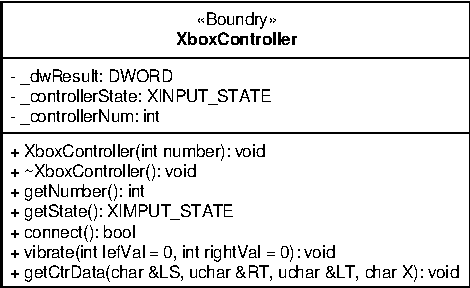
\includegraphics[]{../fig/diagrammer/pc/cd_xboxcontroller.pdf}
\caption{Klassebeskrivelse for boundry-klassen XboxController}
\label{fig:cd_xboxcontroller}
\end{figure}

\textbf{Attributter}

\begin{table}[h]
\begin{tabularx}{\textwidth}{| Z | Z | L{10cm} |} \hline
Navn & Type & Beskrivelse \\\hline
\texttt{\_dwResult}				& \texttt{DWORD}		&Variabel af typen DWORD, skal indeholde data om controllerens tilstand.\\\hline

\texttt{\_controller- State}	& \texttt{XINPUT\_STATE}&Struct af typen XINPUT\_STATE. Indeholder hhv. DWORD, der indeholder en værdi forskellig fra 0 hvis der er sket en ændring i controllerens tilstand, og XINPUT\_GAMEPAD, der indeholder alle værdier som fortæller om controllerens nuværende tilstand.\\\hline

\texttt{\_controller- Num}		& \texttt{int}			&Variabel af typen int der indeholder controller nummer.\\\hline
\end{tabularx}
\caption{Attributter for klassen XboxController}
\label{table:attr_xboxcontroller}
\end{table}

\textbf{Metoder}

\begin{table}[h]
\begin{tabularx}{\textwidth}{| L{2.5 cm} | Z |} \hline
Prototype 	& \texttt{void XboxController(int number)} \\\hline
Parametre 	& \texttt{number} 			\newline Det ønskede controller ID (1-4). \\\hline
Returværdi	& \texttt{void} 			\newline \\\hline
Beskrivelse	& Constructor til klassen XboxController. \newline \\\hline
\end{tabularx}
\caption{Metodebeskrivelse for constructoren af \texttt{XboxController} klassen}
\label{table:met_xboxcontroller}
\end{table}

\clearpage

\begin{table}[h]
\begin{tabularx}{\textwidth}{| L{2.5 cm} | Z |} \hline
Prototype 	& \texttt{void $\sim$XboxController()} \\\hline
Parametre 	& \texttt{void}				\newline \\\hline
Returværdi	& \texttt{void} 			\newline \\\hline
Beskrivelse	& Destructor til klassen XboxController. \newline \\\hline
\end{tabularx}
\caption{Metodebeskrivelse for destructoren af \texttt{XboxController} klassen}
\label{table:met_xboxcontroller_de}
\end{table}

\begin{table}[h]
\begin{tabularx}{\textwidth}{| L{2.5 cm} | Z |} \hline
Prototype 	& \texttt{int getNumber()} \\\hline
Parametre 	& \texttt{void}				\newline \\\hline
Returværdi	& \texttt{int} 				\newline Controllerens ID \\\hline
Beskrivelse	& Denne funktion har til formål at returnere objektets ID. \newline \\\hline
\end{tabularx}
\caption{Metodebeskrivelse for \texttt{getNumber()}}
\label{table:met_getnumber}
\end{table}

\begin{table}[h]
\begin{tabularx}{\textwidth}{| L{2.5 cm} | Z |} \hline
Prototype 	& \texttt{XINPUT\_STATE getState()} \\\hline
Parametre 	& \texttt{void}				\newline \\\hline
Returværdi	& \texttt{XINPUT\_STATE} 	\newline Struct af typen XINPUT\_STATE. Indeholder hhv. DWORD og XINPUT\_GAMEPAD. \\\hline
Beskrivelse	& Denne funktion har til formål at opdatere \_controllerState som indeholder controllerens nuværende tilstand og info om hvorvidt den har skiftet tilstand. \\\hline
\end{tabularx}
\caption{Metodebeskrivelse for \texttt{getState()}}
\label{table:met_getstate}
\end{table}

\begin{table}[h]
\begin{tabularx}{\textwidth}{| L{2.5 cm} | Z |} \hline
Prototype 	& \texttt{bool connect()} \\\hline
Parametre 	& \texttt{void}				\newline \\\hline
Returværdi	& \texttt{bool} 			\newline Controllerens connection tilstand \\\hline
Beskrivelse	&  Denne funktion returnerer hvorvidt der er forbindelse til controlleren. \\\hline
\end{tabularx}
\caption{Metodebeskrivelse for \texttt{connect()}}
\label{table:met_connect}
\end{table}

\clearpage

\begin{table}[h]
\begin{tabularx}{\textwidth}{| L{2.5 cm} | Z |} \hline
Prototype 	& \texttt{void vibrate(int leftVal = 0, int rightVal = 0)} \\\hline
Parametre 	& \texttt{leftVal}			\newline En værdi der fortæller controllerklassen hvor hurtigt vibrater motoren i venstre side af controlleren skal køre (0 - 65535).	\newline \newline
			  \texttt{rightVal}			\newline En værdi der fortæller controllerklassen hvor hurtigt vibrater motoren i højre side af controlleren skal køre (0 - 65535). \\\hline
Returværdi	& \texttt{void} 			\newline \\\hline
Beskrivelse	&  Denne funktion igangsætter højre og venstre vibrater med en styrke alt efter input parameterne leftVal og rightVal. Inputparameterne kan gå mellem 0 og 65535, hvor 0 er ingen vibrering og 65535 er maksimal vibrering. Hvis der ikke gives parametre med i funktionen, vil den automatisk sætte parameterne til 0 og dermed slukke for vibraterne.\\\hline
\end{tabularx}
\caption{Metodebeskrivelse for \texttt{vibrate()}}
\label{table:met_vibrate}
\end{table}

\begin{table}[h]
\begin{tabularx}{\textwidth}{| L{2.5 cm} | Z |} \hline
Prototype 	& \texttt{void getCtrlData(char \&LS, uchar \&RT, uchar \&LT, char X)} \\\hline
Parametre 	& \texttt{LS}				\newline En reference til den char der ønskes at funktionen indsætter data om controllerens ''Left Stick'' tilstand i.				\newline \newline
			  \texttt{RT}				\newline En reference til den unsigned char der ønskes at funktionen indsætter data om controllerens ''Right Trigger'' tilstand i.\newline \newline
			  \texttt{LT}				\newline En reference til den unsigned char der ønskes at funktionen indsætter data om controllerens ''Left Trigger'' tilstand i.\newline \newline
			  \texttt{X}				\newline En reference til den char der ønskes at funktionen indsætter data om controllerens ''X-button'' tilstand i. \\\hline
Returværdi	& \texttt{void} 			\newline \\\hline
Beskrivelse	&  Denne funktion har til formål at returnere nye controller tilstande, for controllerens Left Stick, Right Trigger, Left Trigger og X-button, på de refererede parametres plads.\\\hline
\end{tabularx}
\caption{Metodebeskrivelse for \texttt{getCtrlData()}}
\label{table:met_getctrldata}
\end{table}